\label{chapter:4_differentiable_mrf_inference_for_training_co_solution_predictors}

\todo[inline]{Proposed alternate titles for this contribution : \emph{Learning Combinatorial Optimization Predictors with MRF-based Inference}, \emph{Differentiable MRF Inference for Training CO Solution Predictors}, \emph{Coupling GNNs and MRF Inference for Combinatorial Optimization}, \emph{MRF-augmented Learning for Combinatorial Optimization}, \emph{Belief Propagation-based Training of Graph Neural Predictors for CO}}

\section{Introduction}

Solving large-scale combinatorial optimization (CO) problems remains a challenging task, as exact methods scale poorly and heuristic methods often struggle to balance solution quality with efficiency. Recent work has shown that machine learning, and in particular graph neural networks (GNNs), can be used to learn effective heuristics for CO. In supervised settings, GNN-based models trained on solved instances have been able to predict high-quality solutions or guide solvers toward promising regions of the search space \cite{nair_solving_2020,sun_difusco_2023,li_t2t_2023}. 

A popular line of research encodes mixed-integer linear programs as bipartite graphs connecting decision variables and constraints \cite{gasse_exact_2019}. GNNs operating on these graphs learn embeddings for variables, which are then scored to indicate the likelihood of being set to one in an optimal solution. These scores can be used directly to produce candidate solutions \cite{nair_solving_2020}, or indirectly to guide constructive heuristics \cite{dai_learning_2017,dalle_learning_2022}. While promising, such methods share a common limitation: they predict variable states independently at inference time. This factorized view ignores explicit dependencies between variables, increasing the likelihood of generating infeasible solutions.

Graphical models \cite{koller_probabilistic_2010,wainwright_graphical_2007} provide a natural remedy to this issue. Markov Random Fields (MRFs) explicitly represent dependencies between variables by associating them with nodes in a graph and constraints or relations with factors \cite{wainwright_graphical_2007}. Inference algorithms such as Belief Propagation (BP) or its variants exploit this structure to compute approximate marginals or maximum a posteriori (MAP) assignments. Although exact only on trees, BP has been applied successfully on graphs with cycles in fields such as computer vision \cite{domke_learning_2013} and natural language processing \cite{stoyanov_minimum-risk_2012}. Importantly for our purposes, BP is fully differentiable, allowing gradients to be propagated through inference and enabling end-to-end training with neural architectures.

\todo[inline]{add mention of Mean-Field approximations and like to the background chapter on MRFs}

Our contribution in this chapter is to couple GNN predictors with MRF-based inference in order to better capture dependencies between decision variables. Specifically, we extend the framework of Nair et al.\ \cite{nair_solving_2020} by replacing fully factorized predictions with an exponential-family MRF posterior distribution. The parameters of this distribution are predicted from GNN embeddings of the variable–constraint bipartite graph, and inference is performed using differentiable algorithms such as BP or mean-field. This integration mitigates the risk of producing infeasible solutions, while remaining compatible with gradient-based training.

We demonstrate our approach on the Maximum Independent Set (MIS) and Set Covering (SCP) problems, which serve as canonical NP-hard benchmarks in combinatorial optimization. Empirical results show that incorporating graphical models into the prediction pipeline improves solution quality compared to factorized GNN predictors, highlighting the benefit of modeling explicit dependencies. Beyond MIS and SCP, the framework we propose is broadly applicable to other CO problems, suggesting that graphical-model–augmented predictors can provide a powerful bridge between learned heuristics and structured optimization. 

The contributions presented in this chapter are:(i) An MRF-augmented predictor that replaces factorized scores with structured posteriors predicted by a GNN; (ii) a BP-Guided Decimation (BPGD) decoding strategy that integrates partial assignments as evidence; (iii) empirical gains on MIS (and SCP) versus factorized baselines under fixed-iteration inference. The problems considered are known to be difficult to solve with BP. We will therefore pay particular attention to the space and time costs incurred by these techniques, and investigate the impact of the number of BP iterations and other model hyperparameters on performance.

\subsection{Related work}
Classical works have shown that message-passing algorithms such as \emph{Belief Propagation} (BP) can be applied to combinatorial optimization (CO) by formulating problems as graphical models. For instance, Park and Shin~\cite{park_max-product_2017} demonstrate that the max-product BP algorithm can recover exact solutions for certain linear programming (LP) relaxations of CO problems (e.g., maximum matching, network flow) when the relaxation is tight. While these results establish important theoretical connections between BP fixed points and LP optimality, they rely on strong assumptions such as acyclic or near-tree factor graph structures and do not leverage learning to adapt inference dynamics to more general, loopy problem instances.

More recent research integrates machine learning with BP to improve convergence and inference quality. Deep Attentive Belief Propagation (DABP)~\cite{deng_deep_2022} and related \emph{Belief Propagation Neural Networks} (BPNN)~\cite{kuck_belief_2020} unroll BP iterations into differentiable layers and learn damping factors or message weights using neural networks. These approaches effectively accelerate inference and stabilize loopy BP but still treat BP as a stand-alone inference procedure. In contrast, our framework uses BP not only for inference but also to compute \emph{likelihoods} at training time, thereby providing a fully probabilistic, differentiable model for CO problems.

In parallel, a large body of work has explored the use of \emph{graph neural networks} (GNNs) to learn heuristics for CO without adopting a probabilistic formulation. Examples include the reinforcement-learning approach of Dai et al.~\cite{dai_learning_2017}, the greedy neural combinatorial optimization of Dai et al.~\cite{dai_learning_2017}, and the hybrid GNN--MILP framework of Gasse et al.~\cite{gasse_exact_2019}. These methods treat the GNN as a policy or ranking network that guides a solver (e.g., branch-and-bound) through learned embeddings. While effective, they only capture variable dependencies implicitly through message aggregation and are prone to over-smoothing and sensitivity to hyperparameters. In contrast, our MRF-based formulation captures dependencies explicitly through factor potentials and ensures local consistency of beliefs through BP inference.

Another line of work focuses on \emph{generative} and \emph{sampling-based} approaches to CO. Energy-based models~\cite{grathwohl_oops_nodate,caramanis_optimizing_2023,sun_revisiting_2023}, diffusion models such as \textsc{Difusco}~\cite{sun_difusco_2023}, and differentiable optimization frameworks such as \textsc{InferOpt}~\cite{dalle_learning_2022} aim to learn probability distributions over feasible solutions. While these models achieve strong empirical performance, they often rely on costly black-box solvers during training (perturb-and-MAP sampling), suffer from slow mixing in discrete solution spaces, or require large neural architectures for denoising-based diffusion processes. Our approach avoids these issues by maintaining full differentiability and parallelizability, with tractable likelihood computation via BP rather than Monte Carlo estimation.

Finally, works such as Wiseman et al.~\cite{wiseman_amortized_2019} have investigated learning to stabilize or accelerate BP in challenging inference regimes. Although we do not tackle this direction directly, our framework could naturally incorporate such learned damping or scheduling strategies. Overall, our contribution differs from prior literature by providing a unified probabilistic framework that (i) preserves local distributional consistency through BP inference, (ii) allows likelihood-based end-to-end training without solver-in-the-loop gradients, and (iii) scales efficiently through parallel message passing.





\begin{table}[htbp]
\centering
\caption{Compact overview of representative works linking combinatorial optimization (CO), graphical models, and differentiable inference.}
\label{tab:lit_review_co_mrf_merged}
\small
\setlength{\tabcolsep}{4pt}
\renewcommand{\arraystretch}{1.08}
\begin{tabular}{|p{2.6cm}|p{4.2cm}|p{2.8cm}|p{4.6cm}|}
\hline
\textbf{Authors / Year} & \textbf{Method} & \textbf{Problem Focus} & \textbf{Inference / Gradient Strategy} \\
\hline

\multicolumn{4}{|l|}{\textbf{GNN-based Heuristics}} \\
\hline
\cite{dai_learning_2017} & GNN + RL for heuristic construction & TSP, MVC, MIS & Policy-gradient learning; solver-free rollouts \\
\cite{gasse_exact_2019} & Graph representation of LP + ML for Branch-and-Bound & General ILPs & GNN-learned branching policies \\
\cite{nair_solving_2020} & Neural-guided search for MIP solving & General MIPs / CO & Learned branching and exploration policies; end-to-end reinforcement learning with solver feedback \\
\hline

\multicolumn{4}{|l|}{\textbf{Generative / Energy-based}} \\
\hline
\cite{caramanis_optimizing_2023} & Generative / score-based CO models & General CO & Diffusion or score-based inference \\
\cite{grathwohl_oops_nodate} & Energy-based discrete optimization & General CO & Gradients via contrastive / MCMC estimation \\
\cite{sun_difusco_2023} & Diffusion-guided optimization (DiFusCO) & General CO & Denoising score matching; sampling-based inference \\
\cite{dalle_learning_2022} & Learning distributions over solutions & General CO & Likelihood-based; solver-guided sampling \\
\cite{berthet_learning_2020} & MAP-and-perturb & General CO & Randomized solver perturbations for gradients \\
\hline

\multicolumn{4}{|l|}{\textbf{Learned Belief Propagation}} \\
\hline
\cite{park_max-product_2017} & Max-product BP for LP relaxations & MIS, MVC, matchings & BP convergence and CO equivalence analysis \\
\cite{kuck_belief_2020} & Learned message passing & Graphical models & Trainable damping / message weights \\
\cite{deng_deep_2022} & Deep / neural BP & Discrete models & Unrolled differentiable BP layers \\
\cite{wiseman_amortized_2019} & Amortized inference with BP & Structured prediction & Learned initialization / unrolled inference \\
\hline

\multicolumn{4}{|l|}{\textbf{Proposed Framework (This Thesis)}} \\
\hline
\textbf{Schulz (2025)} & \textbf{MRF-based CO with differentiable BP inference} & \textbf{MIS, MVC} & \textbf{Fully differentiable (sum-/max-product) BP; exact gradients; primal-dual optimization perspective} \\
\hline

\end{tabular}
\end{table}








\section{Proposed framework}
In this section we present the details of our proposed framework, combining GNNs with MRF inference. The central idea is to move beyond fully factorized predictors, which treat variable assignments as independent, and instead define a structured posterior distribution over solutions. This distribution is modeled as an exponential-family Markov Random Field whose parameters are predicted by a GNN encoder operating on a graph representation of the problem. Inference in this MRF—via belief propagation or mean-field approximations—yields marginal distributions that capture dependencies between variables and can be used to guide a greedy solution construction by BP Guided Decimation (BPGD). 

We formalize this approach by first defining the class of CO problems we target, and then specifying how their structure is encoded into the GNN–MRF architecture.

\subsection{Problem class and graph representation}
We focus on the class of combinatorial optimization problems that can be formulated as binary linear programs
\begin{equation}
    (\PROB) \Leftrightarrow 
    \left\{ 
    \begin{array}{ll}
         \max        & \CVEC^\top \XVEC \\
         \text{s.t.} & \AMAT \XVEC \leq \BVEC \\
                     & \XVEC \in \{0,1\}^{\NVAR},
    \end{array}
    \right.
\end{equation}
with cost vector $\CVEC \in \mathbb{R}^n$ and constraints defined by $(\AMAT,\BVEC) \in \R^{\NCONSTR \times \NVAR} \times \R^{\NCONSTR}$. Many classical problems—including Maximum Independent Set, Max-Cut, Matching, and TSP—fit into this family, which we denote by $\ILPFAM$.

In a probabilistic view, a solution $\XVEC$ of problem $(\PROB)$ is a realization of a random variable $\XRAV = (\XRAV_i)_{i=1}^{\NVAR}$ drawn from an unknown distribution $\PDIST^*(\XVEC \mid \PROB)$. The task of learning a predictor is then to approximate $\PDIST^*(\cdot \mid \PROB)$ from training data consisting of solved problem instances.

A widely used approach is to represent $(\PROB)$ as a graph and train a GNN to output variable-level scores $\SCORE_i$, which are interpreted as the likelihood of $\XVEC_i = 1$ \cite{dai_learning_2017,gasse_exact_2019,nair_solving_2020,sun_difusco_2023}. This effectively treats solution prediction as a multivariate binary classification task with factorized distribution
\begin{equation}
    \label{equ:fully_factorized_distribution}
    \PDIST(\XVEC_1,\dots,\XVEC_{\NVAR} \mid \PROB) \approx \prod_{i=1}^{\NVAR} \PDIST(\XVEC_i \mid \PROB),
\end{equation}
where dependencies between variables are only implicitly captured by the GNN encoder. While such models achieve good results, they often produce infeasible solutions because they ignore explicit constraints at inference time. Scores $(\SCORE_i)_{1\leq i\leq \NVAR}$ must therefore be post-processed (e.g.\ through greedy decoding) to yield valid solutions, limiting their effectiveness.

Our contribution is to replace the fully factorized approximation (~\ref{equ:fully_factorized_distribution}) with a structured probabilistic model. Specifically, given the variable–constraint bipartite representation $\VCG=(\VCGV \cup \VCGC, \VCGE)$ of $(\PROB)$ (see Section ~\ref{sec:vcg_definition}
 for details on the construction of $\VCG$), we define a Markov Random Field
\begin{equation}
    \PDIST(\XVEC \mid \PROB) \propto \prod_{\FACTOR \in \VCGC} \POTENTIAL_{\FACTOR}(\XVEC_{\FACTOR};\PROB),
\end{equation}
where each factor $\POTENTIAL_{\FACTOR} : \mathcal{X}_{\FACTOR} \rightarrow \R^+$ encodes the compatibility of variable assignments with constraint $\FACTOR$, and $\XVEC_{\FACTOR}$ denotes the subset of variables involved in that constraint. This formulation allows us to capture dependencies between variables explicitly, with the MRF potentials parametrized by a GNN encoder operating on $H$. Inference in this model—via belief propagation or mean-field—produces approximate marginals that are locally consistent with the problem constraints and can be used directly to construct feasible solutions. 

The reader will notice that in this chapter we treat the variable-constraint bipartite graph representing the problem as the \emph{factor graph} defining the target MRF distribution. This will not necessarily be the case in following works when introducing approximate and more tractable distributions. In this chapter the terms constraint and factor are interchangeable and we will denote the set of factors by $F$ and individual factors as $\alpha$. We would also stress that the graph used as input to the pipeline which serves as a representation of the problem and the factor graph upon which the MRF is defined are two distinct graphs, but in this chapter their structures are identical, we will denote the graph $\VCGFULL$ when working on the graph representation of the problem and $\FGFULL$ when dealing with the factor graph.

Figure~\ref{fig:model_design_nair} shows the baseline GNN predictor of Nair et al.\ \cite{nair_solving_2020}, which assumes a fully factorized distribution. In the following sections, we present our MRF-augmented framework, which generalizes this design by embedding constraint factors into the probabilistic model and performing structured inference at prediction time.

\begin{figure}[h]
    \centering
    \begin{tikzpicture}[
            every node/.style={
                minimum width=1.5em, 
                minimum height=1.5em},
        ]
        \node[draw] (p) {Input $P$};
        \node[draw,right=2cm of p] (gnn) {GNN};
        \node[draw,right=2cm of gnn] (pred) {Prediction $\XVEC\in\{ 0,1 \}^{\NVAR}$};
        \draw (p) -- (gnn) node[midway,label={$\scriptstyle \VCGFULL$}] {};
        \draw (gnn) -- (pred) node[midway,label={$\scriptstyle \SCORE_i, i\in \VCGV$}] {};
    \end{tikzpicture}
    \caption{Model inspired by Nair et al.~\cite{nair_solving_2020}.}
    \label{fig:model_design_nair}
\end{figure}

\paragraph{Maximum Independent Set (MIS) problems} In this first contribution we focus on the classical edge based formulation of the problem defined over an undirected graph $\GFULL$: 
\begin{equation}
    (\MISPROB) \Leftrightarrow \left\{ \begin{array}{clr}
        \max & \mathds{1}^T \XVEC & \\
        \text{s.t.} & \XVEC_i + \XVEC_j \leq 1 & \forall (i,j) \in E
    \end{array}
    \right.
\end{equation}
where the decision variable $x_i$ indicates whether vertex $i$ belongs to the independent set, and the constraints ensure that both endpoints of any edge cannot simultaneously belong to the set.

The corresponding factor graph contains only factors of size $2$. The features provided to the model are extracted by solving the continuous relaxation of $\MISPROB$. Since the trivial solution $\XVEC_i=1/2$ is always optimal for this problem the features essentially do not provide any information about the solution and the feature extraction process must make full use of any topological properties of the graph to learn meaningful information.

\paragraph{Set Covering problems (SCP)} The problem formulation as a linear program is given in standard form : 
\begin{equation}
    (\SCPROB) \Leftrightarrow \left\{ \begin{array}{clr}
        \min & \mathds{1}^T \XVEC & \\
        \text{s.t.} & \sum\limits_{f\in \SETI} \XVEC_f \geq 1 & \forall i \in \ITEMS
    \end{array}
    \right.
\end{equation}

where $x = (x_f)_{f\in\SETI}$ are binary decision variables indicating if set $f$ belongs to the cover, $\SETI \subseteq \SETS$ denotes all sets containing item $i \in \ITEMS$. The constraints, one for each item, ensure that each item belongs to at least one set in the covering.

\subsection{MRF parametrization and exponential family}
For a given problem $(\PROB)$ we consider MRFs defined on a factor graph $\FGFULL$, where $\VCGV$ indexes decision variables and $\FGF$ indexes factors (or constraints). To ground our approach in a well-studied setting, we restrict to the \emph{exponential family}. Each factor $\FACTOR \in \FGF$ has potential
\[
\POTENTIAL_{\FACTOR}(\XVEC_{\FACTOR}) = \exp\!\left(\langle \EPARAM_{\FACTOR}, \SSTAT_{\FACTOR}(\XVEC_{\FACTOR}) \rangle \right),
\]
so that the overall distribution is
\begin{equation}
    \PDIST_{\EPARAM}(\XVEC \mid \PROB) \propto \exp \!\left( \langle \EPARAM, \SSTAT(\XVEC) \rangle \right),
\end{equation}
with $\EPARAM = (\EPARAM_{\FACTOR})_{\FACTOR \in \FGF}$ the parameters and $\SSTAT(\XVEC) = (\SSTAT_{\FACTOR}(\XFACT) )_{\FACTOR\in \FGF}$ the sufficient statistics and with $\SSTATF(\XFACT), \EPARAMF \in \R^{\FDIM}$. The parameter dimension is $\SSDIM = \sum_{\FACTOR} \FDIM_{\FACTOR}$, where $\FDIM_{\FACTOR}$ denotes the number of parameters of factor $\FACTOR$. Training consists of learning $\EPARAM \in \EPARAMDOM = \mathbb{R}^{\SSDIM}$ such that $\PMRF$ matches the desired distribution over solutions.

\paragraph{Choosing the sufficient statistics} As a choice for the \emph{sufficient statistics} we chose the \emph{canonical over-complete representation} ~\cite{wainwright_graphical_2007} (see Chapter ~\ref{sec:mrf_intro}). For each factor $\FACTOR$ there are $\FDIM_{\FACTOR} = 2^{|\FACTOR|}$ possible configurations $\XFACT$ and the same number of corresponding parameters $\EPARAM_{\FACTOR}(\XFACT)$. The total number of parameters of the MRF corresponding to a problem $(\PROB)$ is $d$. Factor configurations $\XFACT$ that are feasible with regards to the constraint $\FACTOR$ are expected to have higher corresponding $\EPARAM(\XFACT)$ than those that violate the constraints, thus pushing the probability of all assignments corresponding to feasible solutions higher than those that violate the constraint.

Each problem $(\PROB)$ must be mapped to its set of parameters $\EPARAM(\PROB)$; this is the role of the \emph{parameter prediction head} of the proposed framework. From an implementation point of view it is important to note the bottleneck incurred from the choice of sufficient statistics. The number of parameters increases exponentially with the size of the largest factor in the graph. This motivates our choice of problems whose formulations yield a controllable factor size. In the edge-based formulation of MIS, all factors involve exactly two variables, whereas for SCP we construct instances according to a procedure that guarantees each item is covered by exactly $k$ sets (with $k$ chosen to be small). In the next chapter, we address problems involving larger factors and introduce strategies to handle the increased computational complexity.

\todo[inline]{The canonical over-complete representation should probably be presented in the background chapter on MRFs}

\subsection{Neural parameter predictor} The following details the implementation of the neural network used to predict the set of canonical parameters of problem $(\PROB)$. Our predictor combines two components:
\begin{enumerate}
    \item \textbf{Graph encoder.} A multi-layer GNN operating on the variable–constraint bipartite graph computes embeddings $\EMB_u \in \mathbb{R}^{\EMBDIM}$ for each vertex $u \in \VCGV \cup \VCGC$. This serves as feature extraction from the structured problem representation.
    \item \textbf{Parameter predictor.} Given embeddings of variables connected to factor $\FACTOR$, a differentiable function $\FPARAMPRED_{\FACTOR}$ produces $\EPARAM_{\FACTOR}$, the canonical parameters of the factor potential:
    \[
    \EPARAM_{\FACTOR} = \FPARAMPRED_{\FACTOR}(\EMB_{\FACTOR}).
    \]
\end{enumerate}
The predicted parameter set $\EPARAM$ defines the MRF posterior. Figure~\ref{fig:model_design_efcanonicalparam} illustrates this architecture.

\paragraph{Graph encoder} A problem $(\PROB)$ is represented as its variable-constraint bipartite graph $\VCGFULL$ (where $\VCGV$ indexes the set of decision variables and $\VCGC$ the set of constraints) and by a set of features $\FEATURES = \{ \FEATURES_u \}_{u \in \VCGV \cup \VCGC}$. The graph encoder is a parametrized differentiable function that converts the structured representation of the problem into a set of vector embeddings $\EMB = \{ \EMB_u \}_{u \in \VCGV \cup \VCGC }$ that will serve as inputs to the following components of the predictor. We denote the set of trainable parameters of the graph encoder $\GNNEMB$ by $\GNNEMBPARAM$.
\begin{equation}
    \GNNEMB ( \VCG, \FEATURES; \GNNEMBPARAM) = \EMB
\end{equation}

In practice $\GNNEMB$ is defined as a sequence of $\NUMGNNLAYERS$ graph convolution layers (see experimental results for details on the GNN implementation). 



\paragraph{Parameter prediction head} The parameter prediction head's role is to transform the set of vertex embeddings $\EMB$ resulting from the graph encoder into a set of canonical parameters $\EPARAM(\EMB)$. We will denote this function as $\FPARAMPRED$ and its set of trainable parameters $\FPARAMPREDPARAM$. For each factor size in the factor graph $k \in \{ 1, ..., \max_{\FACTOR \in \VCGC} |\FACTOR| \}$ we define a predictor $\FPARAMPRED_{k} : \R^{\EMBDIM} \rightarrow \R^{2^k}$ and the final parameter vector is obtained as 
\begin{equation}
    \EPARAM  = \{ \FPARAMPRED_{|F|} (\FEMB) \}_{\FACTOR\in \VCGC}
\end{equation}

\subsection{Differentiable inference}

Once parameters are predicted, inference in the MRF provides structured predictions. Depending on the task, we may:
\begin{itemize}
    \item compute a MAP solution via max–sum BP,
    \item compute approximate marginals via sum–product BP (used during training),
    \item or perform conditional inference when partial assignments are known, e.g.\ in BP guided decimation.
\end{itemize}
Inference thus bridges learning and optimization, ensuring that predictions take into account variable dependencies.

It is worth noting the conceptual similarities with recent approaches that integrate combinatorial optimization problems as layers within machine learning models \citep{berthet_learning_2020, dalle_learning_2022}. In these works, the optimization layer is treated as a black box: logits or continuous parameters are passed to a state-of-the-art solver that computes exact (but non-differentiable) solutions, while gradient information is approximated by sampling or perturbing the inputs to estimate the sensitivity of the outputs. In contrast, we propose to use BP as the inference mechanism. BP performs approximate but fully differentiable message passing, defining a smooth energy-based distribution over feasible solutions. If BP inference were exact, it would recover the same optimal solutions as the underlying combinatorial optimization solver, while remaining amenable to end-to-end training and efficient parallelization.

At this stage we have computed the set of canonical parameters that correspond to problem $(\PROB)$ and denote them $\EPARAM(\PROB)$. Depending on the task at hand, we need to solve an inference problem; for training we might be interested in the full joint distribution $\PDIST_{\EPARAM(\PROB)}$, the factor marginals $\FMARGIN$ or some conditional distribution. We propose to leverage the fully differentiable nature of the message passing BP schemes to solve this problem and train the model in a end-to-end manner. 

Two inference methods are investigated in this contribution: Loopy Belief Propagation (LBP) and Naive Mean-Field (NMF) (see Chapter ~\ref{sec:mrf_intro} for details and implementation details for both algorithms). The notable side of this choice of inference method is the capability of the inference method to capture the dependencies that exist between variable as well as the possibility of tailoring the values of the canonical parameters $\EPARAM$ to partial evidence acquired while solving the problem. This aspect will be further discussed in the following subsection on Guided Decimation techniques.

Messages and marginals computed by BP (or NMF) are the result of fully differentiable operations and do not add any further parameters to the model. Being an iterative procedure and since we have no guarantee of convergence we fix the maximum number of iterations to a fairly low number and add damping of the messages \cite{heskes_uniqueness_2004,wainwright_graphical_2007,meltzer_convergent_2012}. 

\subsection{Solution decoding}
Having predicted the parameters $\EPARAM(P)$ of the distribution the task is now to retrieve a solutions to the problem $(P)$. We give here a description of methods for decoding solutions of the problem by leveraging the information provided by the distribution $\PMRF$.

\subsubsection{General case}
We can exploit approximate inference via Belief Propagation (BP) to guide enumeration strategies such as diving or Branch‑and‑Bound in combinatorial optimisation. In each node of the search tree (or each dive step) some decisions have been made and others remain free: BP can be conditioned on the fixed decisions so far to compute approximate marginal or conditional distributions over the remaining variables. One can then use these distributions as heuristics for selecting the next variable to branch on (or fix in a dive), choosing for instance the variable with the greatest entropy, largest deviation from uniformity, or highest probability of being in the optimal solution. This yields a search strategy that is informed by the structure of the problem and the partial evidence seen so far, rather than relying solely on static heuristic rules. Prior work in constraint programming has shown that beliefs from BP-style propagation can indeed guide branching heuristics effectively. In our case, we propose to integrate BP more directly as a fully differentiable module, so that the branching or diving decisions can themselves benefit from gradient-based tuning and end-to-end learning.


\begin{figure}[H]
\centering
\begin{tikzpicture}[
  font=\footnotesize, >=latex,
  var/.style={circle, draw, minimum size=5mm, inner sep=0pt},
  varfix/.style={circle, draw, fill=gray!30, minimum size=5mm, inner sep=0pt},
  fac/.style={rectangle, draw, minimum size=3mm, inner sep=1pt},
  box/.style={rounded corners, draw, inner sep=3pt},
  legendbox/.style={draw, rounded corners, inner sep=2pt}
]

% (a) Conditioned factor graph
\node[box, minimum width=3.8cm, minimum height=2.1cm] (G) {};
\node at ([yshift=1.2cm]G.north) {\textbf{(a) Conditioned graph}};

\node[varfix] (x1) at ([xshift=-1.2cm,yshift=0.4cm]G.center) {$x_1$};
\node[var]    (x2) at ([xshift= 0.0cm,yshift=0.4cm]G.center) {$x_2$};
\node[var]    (x3) at ([xshift= 1.2cm,yshift=0.4cm]G.center) {$x_3$};
\node[var]    (x4) at ([xshift=-0.6cm,yshift=-0.5cm]G.center) {$x_4$};
\node[varfix] (x5) at ([xshift= 0.9cm,yshift=-0.5cm]G.center) {$x_5$};

\node[fac] (f12) at ([xshift=-0.6cm,yshift=0.0cm]G.center) {};
\node[fac] (f23) at ([xshift= 0.6cm,yshift=0.0cm]G.center) {};
\node[fac] (f24) at ([xshift=-0.2cm,yshift=-0.2cm]G.center) {};
\node[fac] (f35) at ([xshift= 0.9cm,yshift=-0.2cm]G.center) {};

\draw (x1)--(f12)--(x2);
\draw (x2)--(f23)--(x3);
\draw (x2)--(f24)--(x4);
\draw (x3)--(f35)--(x5);

% BP box
\node[box, right=8mm of G, align=center] (BP) {BP on\\ fixed graph};
\draw[->, thick] (G) -- (BP);

% marginals + selection
\node[box, right=8mm of BP, align=left] (SEL) {cond.\ marginals $\Rightarrow$ select $x_2$};
\draw[->, thick] (BP) -- (SEL);

% (b) Branch step (tiny tree)
\node at ([yshift=1.2cm]SEL.north) {\textbf{(b) Guided branching}};
\node[box, right=8mm of SEL, align=center, inner sep=2pt] (NODE) {$x_1{=}0,\,x_5{=}1$};
\node[box, below left=5mm and 4mm of NODE, inner sep=2pt] (L) {$x_2{=}0$};
\node[box, below right=5mm and 4mm of NODE, inner sep=2pt] (R) {$x_2{=}1$};
\draw[->, thick] (SEL) -- (NODE);
\draw[->, thick] (NODE) -- (L);
\draw[->, thick] (NODE) -- (R);

%----- Legend ------------------------------------------------------------------
%\node[legendbox, below=12mm of SEL, align=left] (leg) {
%\begin{tabular}{@{}ll@{}}
%\raisebox{0.6ex}{\tikz{\node[varfix, minimum size=3mm]{};}} & fixed variable\\
%\raisebox{0.6ex}{\tikz{\node[var, minimum size=3mm]{};}} & free variable\\
%\raisebox{0.6ex}{\tikz{\node[draw, rectangle, minimum width=3mm, minimum height=3mm]{};}} & factor/constraint \\
%\raisebox{0.6ex}{%
%  \tikz[baseline=-0.5ex]{\draw (0,0) rectangle (3mm,3mm);}}& hh
%\end{tabular}
%};

\node[varfix, below=12mm of G, minimum size=3mm] (varfix_legend) {};
\node[right=2mm of varfix_legend, align=left]   (varfix_legend_label) {Fixed variable};
\node[var, right=of varfix_legend_label, minimum size=3mm] (var_legend) {};
\node[right=2mm of var_legend, align=left]   (var_legend_label) {Free variable};
\node[fac, right=of var_legend_label, minimum size=3mm] (fac_legend) {};
\node[right=2mm of fac_legend, align=left]   (fac_legend_label) {Factor/constraint};

\end{tikzpicture}
\caption{Run BP on the factor graph conditioned by current fixes to obtain conditional marginals over free variables; use them to select the next branching/diving variable and split.}
\end{figure}

\paragraph{Diving Procedures for MIS and SCPs}
Diving procedures are constructive heuristics that iteratively fix variables to feasible values while maintaining problem consistency. In the MIS problem, each dive corresponds to selecting a vertex to include in the independent set; once a vertex is added, all its adjacent vertices are removed from further consideration, thereby enforcing the independence constraint. 
Conversely, in the SCP, diving can proceed by either fixing sets that must belong to the cover—such as when a set is the only one covering a specific element—or by discarding redundant sets that do not cover any new elements. These local decisions reduce the problem size progressively and enable exploring promising partial solutions before full branching or backtracking is applied.

\begin{figure}[H]
\centering
\begin{tikzpicture}[
  v/.style={circle,draw,thick,minimum size=6mm,inner sep=0pt},
  sel/.style={circle,draw,thick,fill=green!25,minimum size=6mm,inner sep=0pt},
  rem/.style={circle,draw,thick,fill=gray!25,minimum size=6mm,inner sep=0pt,opacity=0.9},
  item/.style={rectangle,draw,thick,minimum width=6mm,minimum height=4mm,inner sep=0pt},
  set/.style={rounded corners,draw,thick,inner sep=3pt},
  every edge/.style={draw,thick},
  >=Latex
]

% --- (A) MIS diving (left) ---
\begin{scope}[xshift=-3.2cm]
  \node[align=center,anchor=south] at (0,1.8) {\bf MIS dive};

  % Graph layout (pentagon)
  \node[v]   (a) at (90:1.1)  {$a$};
  \node[v]   (b) at (18:1.1)  {$b$};
  \node[v]   (c) at (-54:1.1) {$c$};
  \node[v]   (d) at (-126:1.1){$d$};
  \node[v]   (e) at (162:1.1) {$e$};

  % Edges
  \draw (a)--(b)--(c)--(d)--(e)--(a) (b)--(d) (c)--(e);

  % Pick vertex b, remove its neighbors a,c
  \node[sel] at (b) {$b$};
  \node[rem] at (a) {$a$};
  \node[rem] at (c) {$c$};

  % Cross out neighbors
  \foreach \x in {a,c}{
    \draw[red,thick] ($(\x)+(-.18,.18)$) -- ($(\x)+(.18,-.18)$);
    \draw[red,thick] ($(\x)+(.18,.18)$) -- ($(\x)+(-.18,-.18)$);
  }

  % Legend box below
  \begin{scope}[yshift=-2.0cm]
    \node[draw,rounded corners,inner sep=3pt,fill=white] (leg) at (0,0) {
      \begin{tabular}{@{}ll@{}}
        \tikz{\node[sel,minimum size=4mm]{};} & selected vertex \\
        \tikz{\node[rem,minimum size=4mm]{};} & removed neighbor
      \end{tabular}
    };
  \end{scope}
\end{scope}

% --- (B) SCP diving (right) ---
\begin{scope}[xshift=3.8cm]
  \node[align=center,anchor=south] at (0,1.8) {\bf SCP dive};

  % Items (top row)
  \foreach \i/\x in {1/-1.6,2/-0.8,3/0.0,4/0.8,5/1.6}{
    \node[item] (i\i) at (\x,1.0) {$a_{\i}$};
  }

  \node[above=2pt of i1, text=green!60!black] {\small \checkmark};
  \node[above=2pt of i2, text=green!60!black] {\small \checkmark};

  % Sets (bottom row)
  \node[set,fill=gray!10]  (S1) at (-1.2,0.0) {\small $\SET_1$};
  \node[set,fill=green!20] (S2) at ( 0.0,0.0) {\small $\SET_2$};
  \node[set,fill=gray!10]  (S3) at ( 1.2,0.0) {\small $\SET_3$};

  % Incidence edges
  \draw (S1.north) -- (i1.south);
  \draw (S1.north) -- (i2.south);
  \draw (S2.north) -- (i2.south);
  \draw (S2.north) -- (i3.south);
  \draw (S2.north) -- (i5.south); % unique coverage of e5
  \draw (S3.north) -- (i3.south);
  \draw (S3.north) -- (i4.south);

  % Annotations

  \begin{scope}[yshift=-2.0cm]
    \node[draw,rounded corners,inner sep=3pt,fill=white] (leg) at (0,0) {
      \begin{tabular}{@{}l@{}}
        \tikz{\node[align=left,anchor=west] at (2.0,0.0) {\small \textbf{add} $\SET_2$  \small (unique cover of $e_5$)};} \\
        \tikz{\node[align=left,anchor=east] at (-2.0,0.0) {\small \textbf{discard} $\SET_1$  \small (no new items)};}
      \end{tabular}
    };
  \end{scope}
\end{scope}

\end{tikzpicture}
\caption{Diving steps: (left) MIS—select a vertex and remove its neighbors; (right) SCP—add a set with unique coverage and discard sets adding no new items.}
\end{figure}

\subsubsection{BP-Guided Decimation (BPGD)}
At inference time we test two ways of sampling solutions of the problem; either by guiding a greedy solver by providing the per-variable marginal distribution values (higher probability results in higher chance of the variable being picked), and a BP-Guided Decimation technique that is a greedy procedure in which the gathered evidence (partial solution at the current iteration) is used to update the per-variable marginal distributions. 

At iteration $t$ a mask of the sufficient statistics vector is computed corresponding to all factor assignments that are incompatible with the current partial solution. For example if $x_1 = 1, x_2=0$ in the current partial solution and there is a factor containing variables $(1,2,3)$ then assignments $(0,0,0), (0,0,1), (0,1,0), (0,1,1), (1,1,0), (1,1,1)$ are all incompatible with known evidence. By setting $\EPARAM(\XFACT) = -\infty$ (or a large negative number in practice) for all incompatible $\XFACT$ values we force the model to assign $0$ probability to those configurations of the solution space. By performing this at each step we increase the probability over all feasible assignments and guide the greedy variable selection process towards good quality solutions. The outline of the algorithm is given in Algorithm ~\ref{alg:bp_guided_decimation}.

Whereas predicting scores with the GNN does not provide any way of integrating partial assignments into the marginal calculations, MRFs do. As we are building a solution we can incorporate the partial solution as evidence into the inference process to update the marginals used at the following steps of the solution construction. This method we refer to as BP Guided Decimation (BPGD) and the details are given in Algorithm ~\ref{alg:bp_guided_decimation}.

\begin{figure}[htbp]
  \centering
  \begin{minipage}{.7\linewidth}
    \begin{algorithm}[H]
        \LinesNumbered
        \caption{BP Guided Decimation}\label{alg:bp_guided_decimation}
        \KwData{$\PROB$, MRF parameters $\EPARAM$}
        \KwResult{Solution $\XVEC$}
        $S \gets$ initialize empty solution \;
        \While{Solution incomplete}{
            Sample new candidate and value $i,\XVEC_i$ from $ \PMRF(\XRAV_i=\XVEC_i | S)$ \;
            Add $\XVEC_i$ to solution \;
            Update set of candidate variables \;
        }
    \end{algorithm}
    \end{minipage}
\end{figure}

The candidate selection process and update of the candidate set depends on the type of problem we are solving. By replacing the $\argmax$ operation by a random sampling from $\PMRF(\XRAV_i | S)$ we can generate a random feasible solution of the problem. As evidence is accumulated throughout the run the probability mass accumulates around feasible solutions in which the desired partial solution is fixed. 

BPGD helps to address a pitfall of score guided greedy algorithm that arises in tie-breaking situations. Two variables may be highly promising but mutually exclusive candidates for the solution (in SCPs two sets may have large coverage but share a large number of items). The greedy solution construction can be tempted to select these two variables because there is no way of updating the scores based on previous selections. This leads to very poor solutions.

On the other hand, performing an inference step at each variable selection is costly on its own. We propose to investigate the performance of BPGD when either by skipping iterations (run inference every $k$ steps) or by triggering updates when the marginal entropy exceeds a threshold.



\subsection{Training objective}
Denote the set of trainable parameters $\TRPARAM = (\GNNEMBPARAM, \FPARAMPREDPARAM)$. We train the model in a supervised learning setting: given a dataset of instances and ground-truth solutions $\mathcal{D} = {(\PROB_i,\YVEC_i)}$, we optimize
\begin{equation}
\TRPARAM^* = \argmin_{\TRPARAM} \ \mathbb{E}_{(\PROB,\YVEC)\in \mathcal{D}} \big[ \LOSSF(\PDIST_{\EPARAM(\PROB;\TRPARAM)}, \YVEC) \big],
\end{equation}
with the loss defined as the average per-factor negative log-likelihood
\begin{equation}
\LOSSF(p_{\EPARAM(\PROB;\TRPARAM)},\YVEC)
= -\frac{1}{|\VCGC|} \sum_{\FACTOR\in\VCGC} \log \FMARGIN(\YVEC_{\FACTOR}; \EPARAM(\PROB;\TRPARAM)),
\end{equation}
where $\FMARGIN(\YVEC_{\FACTOR}) = \PMRF(\XRAV_{\FACTOR} = \YVEC_{\FACTOR})$ are the factor marginals returned by the inference procedure.

\paragraph{Why this loss?}
This choice of loss is attractive because it is tractable and naturally resembles a multi-class classification problem per factor. Each factor $\FACTOR$ defines a local prediction task: select the correct configuration $\YVEC_{\FACTOR}$ among the $2^{|\FACTOR|}$ possibilities. By summing over factors, the training objective encourages the model to assign high probability to locally consistent configurations, without requiring normalization over the full exponential solution space. Unlike the global likelihood, this factor-wise loss can be evaluated using approximate marginals from inference, making it suitable for gradient-based training.

\paragraph{LBP versus NMF.}
The form of the loss depends on the inference method. With LBP, marginals exist over factors of arbitrary arity (e.g., pairwise constraints in MIS or higher-order covering constraints in SCP), so supervision takes the form of multi-class predictions at the factor level. By contrast, NMF assumes a fully factorized distribution, where the only available marginals are variable marginals. In that case, the loss reduces to independent binary classification objectives per variable, which is simpler but ignores higher-order structure. This difference explains why LBP-based training can leverage richer dependencies and typically achieves stronger empirical performance than NMF-based training.

\paragraph{Relation to maximum likelihood.}
The natural training target is to minimize the global negative log-likelihood (NLL) of the MRF:
\begin{equation}
\mathcal{L}_{\text{NLL}}(\TRPARAM)
= -\log \PMRF(\YVEC \mid \PROB;\TRPARAM).
\end{equation}
However, this requires computing the partition function $Z(\EPARAM)$ of the MRF, which is intractable for loopy graphs. Our factor-wise loss serves as a surrogate that bypasses this bottleneck. A principled alternative is to approximate the likelihood using variational free energy methods such as the Bethe free energy, which provide tractable approximations consistent with loopy BP. Exploring such objectives is a promising avenue for future work.

\paragraph{Limitations.}
A key limitation of the factor-wise loss is that it enforces consistency only locally, at the level of individual factors, without guaranteeing global coherence across the full assignment space. In particular, marginals predicted for different factors may not correspond to any valid joint distribution. While BP partially mitigates this by enforcing local consistency during message passing, the lack of a true likelihood objective means the model may overfit to local patterns that do not translate into improved global solutions. Addressing this limitation through likelihood approximations or structured regularization remains an open direction.

\begin{figure}[h!]
    \centering
    \begin{tikzpicture}[
            every node/.style={minimum width=1.5em, minimum height=1.5em}]
        \node[draw] (p) {Input $\PROB$};
        \node[draw,right=1cm of p] (gnn) {GNN};
        \node[right=2cm of gnn] (efcpdots) {$\hdots$};
        \node[draw,above=of efcpdots] (efcp1) {$\FPARAMPRED_{\FACTOR_1}(\cdot)$};
        \node[draw,below=of efcpdots] (efcpK) {$\FPARAMPRED_{\FACTOR_{|\VCGC|}}(\cdot)$};
        \node[draw,right=2cm of efcpdots] (concat) {Concat};
        \node[draw,right=of concat] (mrf) {MRF};
        \draw[->] (p) -- (gnn) node[midway,label={$\scriptstyle \VCGFULL$}] {};
        \draw[->] (gnn.east) -- (efcpdots.west);
        \draw[->] (efcp1.east) -| (concat.west);
        \draw[->] (efcpK.east) -| (concat.west);
        \draw[->] (efcpdots.east) -- (concat.west);
        \draw[->] (concat.east) -- (mrf.west) node[midway,label={$\scriptstyle \EPARAM \in \EPARAMDOM$}] {};
    \end{tikzpicture}
    \caption{GNN feature extraction and MRF parameter prediction.}
    \label{fig:model_design_efcanonicalparam}
\end{figure}

\section{Experiments}
In this section we present experimental results of our pipeline applied to two categories of synthetic CO problems (MIS and SCP). We will first provide an overview of the experimental setup; i.e. model hyperparameter choices, optimizer used, number of epochs and hardware specifications used for training and testing. Then we will present the choices of features and method of extraction and finaly present the results and discussions.

\subsection{Experimental setup} 
All models were implemented using four-layer Graph Convolutional Networks \cite{kipf_semi-supervised_2017} with hidden dimension $\EMBDIM=64$. This choice was made mainly for space constraint motivated reasons. We want to show that MRF-augmented learning methods outperform the basic logit prediction. The models were trained using the Adam optimizer with a learning rate of $10^{-6}$ across all models and datasets. BP (both LBP and NMF) iterations were capped at $10$ iterations maximum, and LBP message damping coefficient was set to $0.5$. Each dataset was split into train/validation/testing sets following a $80/10/10\%$ split.

 The baseline (GNN) outputs logits $\SCORE_i$ for each variable, at test time those scores are used to guide the solution decoder. In the MRF-based models, embeddings $\EMB_u$ for each node $u \in \VCGV \cup \VCGC$ are mapped by MLPs $\FPARAMPRED_k : \mathbb{R}^{\EMBDIM} \rightarrow \mathbb{R}^{2^k}$ (with $k \in \{ 1, ..., \max_{\FACTOR \in \VCGC} |\FACTOR|\}$ the factor sizes) to canonical parameters $\EPARAM_{\FACTOR}$. These parameters are then used by Loopy Belief Propagation (LBP) or Naive Mean-Field (NMF) inference to obtain marginals. For both LBP and NMF models test instances are solved once using the greedy solver guided by the computed variable marginals and using GD.  Three values of RNG seed in $\{2023,2024,2025\}$ are tested for each architecture.

 All experiments were conducted on the Jean Zay supercomputer (IDRIS, France) using a single NVIDIA Tesla V100 (32 GB HBM2) GPU and one CPU core from an Intel Cascade Lake processor. 

\todo[inline]{Move this line to thanks ? \emph{This work was granted access to the HPC resources of IDRIS under the allocation 2025-AD011015229R1 made by GENCI.}}





\paragraph{Note on inference.} 
Since the factor graphs considered here are loopy, standard BP is not guaranteed to converge. In practice, we therefore run BP for a fixed number of iterations, following common practice in loopy BP applications \cite{yedidia_understanding_2003}. While this ensures tractability, it also means that the resulting marginals are only approximate. Nevertheless, our experiments show that even with fixed-iteration inference, solution quality improves substantially compared to factorized baselines.

\subsection{Dataset and instance generation} In this section we give details on the dataset generation process used for preparing data for training and testing within our proposed framework. We focus on two classes of binary variable optimization problems for which: (i) the LP formulation of the problem is compact, (ii) a simple greedy construction policy is known, (iii) the sizes of the factors (number of variables appearing in each constraint) are controllable. Instances are solved using either a simple B\&B solver or, when available, a specialized solver.

\paragraph{MIS} MIS instances were generated using the Erdős–Rényi model for generating random graphs with an edge probability of $15\%$. Three size categories were used $\NVAR = 100, \NVAR\sim \mathcal{U}[200,300], \NVAR\sim \mathcal{U}[700,800]$. For graphs greater than $100$ vertices we capped the degree of nodes at $15$. Labels were produced by solving the problems with KaMIS solver \cite{lamm_finding_2017}.

\todo[inline]{Make sure number of connected components is 1 in all instances }

\paragraph{SCP} SCP problems were generated by using a balanced randomized process in which the item-set adjacency matrix was generated at random for a fixed number of sets and items. We then ensure that there are no empty sets and that each item is covered by $k$ sets. The generated instances are $n=50, m=50, k=5$ and $n\sim\mathcal{U}[200,300], m\sim\mathcal{U}[120,150], k=5$. Labeling was obtained by solving the problem with the CBC solver \cite{greenberg_cbc_2005}.

\todo[inline]{More details on the generation procedure for SCP problems needed ?}

\paragraph{Features} Each problem's continuous relaxation was solved and the features were extracted from the solution including dual values, slack values, status of the basis etc... The full list of features are presented in Table ~\ref{tab:mis_dataset_features}.

\begin{table}
  \centering
\resizebox{\textwidth}{!}{
\begin{tabular}{ |c|l| } 
 \hline
\textbf{Tensor} & \textbf{Feature} \\
\hline
\multirow{4}{*}{Constraints} & Cosine similarity with objective. \\
                             & Slack value, normalized with constraint coefficients. \\
                             & Tightness indicator in LP solution. \\
                             & Dual solution value, normalized. \\
\hline
Edges                        & Constraint coefficient, normalized per constraint. \\
\hline
\multirow{7}{*}{Variables}   & Objective coefficient, normalized. \\
                             & Solution value equals lower bound. \\
                             & Solution value equals upper bound. \\
                             & Solution value (fractional). \\
                             & Simplex basis status (lower, basic, upper, zero) as a one-hot encoding. \\
                             & Reduced cost, normalized. \\
                             %& Fractional value, normalized \\
 \hline


\end{tabular}
}
 \caption{Input variable, constraint and edge features taken from the solution of the continuous relaxation of the problem.}
\label{tab:mis_dataset_features}
\end{table}



\subsection{Results}
Tables~\ref{tab:lbp_nmf_bpgd_test_gap_results} and ~\ref{tab:lbp_nmf_bpgd_test_time_results} report average optimality gaps. Across all datasets, both LBP+BPDG and NMF+BPDG consistently outperform the baseline predictor. Guided decimation yields the best solution quality but requires higher runtime, while greedy decoding is faster but less accurate. Test metrics are averaged over the testing set.

\begin{table}[htbp]
\centering
\resizebox{\textwidth}{!}{
% S columns align numbers on the decimal and on the uncertainty (\pm)
\begin{tabular}{l
                    S[table-format=2.3(2.3)]
                    S[table-format=2.3(2.3)]
                    S[table-format=2.3(2.3)]
                    S[table-format=2.3(2.3)]
                    S[table-format=2.3(2.3)]}
        \toprule
        Dataset & {GNN} & {LBP} & {LBP$+$GD} & {NMF} & {NMF$+$GD} \\
        \midrule
        $SCP\,(n=50, m=50, k=5)$           & 19.919 (11.135) & 8.227 (7.762)  & {\bfseries 1.540 (3.642)} & 12.100 (9.399) & 80.953 (19.535)  \\
        $SCP\,(n\sim \mathcal{U}[100,150], m\sim\mathcal{U}[80,120], k=5)$  & 25.994 (10.995) & 8.470 (5.379) & {\bfseries 1.915 (2.437)} & 12.378 (6.087) & 88.049 (13.123)  \\
        $MIS\,(n=100, p=0.15)$             & 14.553 (5.528)  & 8.853 (4.910)  & {\bfseries 6.921 (8.952)} & 10.194 (4.709) & 23.785 (6.623) \\
        $MIS\,(n\sim [200,300], p=0.15)$   & 22.851 (3.787)  & 20.249 (4.068) & {\bfseries 4.705 (2.982)} & 21.191 (3.678) & 25.254 (3.769) \\
        %$MIS\,(n\sim [700,800], p=0.15)$   &  &  &  &  &  \\
        \bottomrule
    \end{tabular}}
\caption{Average optimality gap (\%) across problem instances for each inference–decoding method. Reported values correspond to GNN-only inference, LBP with greedy decoding, LBP with guided decimation (GD), NMF with greedy decoding, and NMF with guided decimation. Lower values indicate better solution quality. The guided decimation approach (LBP+GD) consistently yields the smallest optimality gaps.}
\label{tab:lbp_nmf_bpgd_test_gap_results}
\end{table}

\begin{table}[htbp]
\centering
\resizebox{\textwidth}{!}{
% S columns align numbers on the decimal and on the uncertainty (\pm)
\begin{tabular}{l
                    S[table-format=2.3(2.3)]
                    S[table-format=2.3(2.3)]
                    S[table-format=2.3(2.3)]
                    S[table-format=2.3(2.3)]
                    S[table-format=2.3(2.3)]}
        \toprule
        Dataset & {GNN} & {LBP} & {LBP$+$GD} & {NMF} & {NMF$+$GD} \\
        \midrule
        $SCP\,(n=50, m=50, k=5)$           & {\bfseries 0.060 (0.380)} & 0.200 (0.130) & 0.404 (0.130) & 0.162 (0.142) & 0.393 (0.143) \\
        $SCP\,(n\sim \mathcal{U}[100,150], m\sim\mathcal{U}[80,120], k=5)$  & {\bfseries 0.156 (0.125)} & 0.463 (0.286) & 0.918 (0.294) & 0.332 (0.179) & 0.849 (0.200) \\
        $MIS\,(n=100, p=0.15)$             & 0.380 (0.166) & 0.423 (0.144) & 0.852 (0.162) & {\bfseries 0.263 (0.142)} & 0.593 (0.143) \\
        $MIS\,(n\sim [200,300], p=0.15)$   & 0.984 (0.264) & 1.015 (0.199) & 2.083 (0.299) & {\bfseries 0.841 (0.220)} & 1.819 (0.292) \\
        %$MIS\,(n\sim [700,800], p=0.15)$   &                 &  &  &  &  \\
        \bottomrule
    \end{tabular}
    }
\caption{Average runtime (in seconds) of the evaluated inference–decoding pipelines across different problem instances. Reported values correspond to GNN-only inference, LBP with greedy decoding, LBP with guided decimation (GD), NMF with greedy decoding, and NMF with guided decimation. Preprocessing time is excluded. The guided decimation variants require multiple inference passes and are therefore significantly slower.}
\label{tab:lbp_nmf_bpgd_test_time_results}
\end{table}

\subsubsection{Train-less inference} As a point of reference it is important to compare results in Table ~\ref{tab:lbp_nmf_bpgd_test_gap_results} with the optimality gap one can expect when solving the problem with guided decimation without learning to predict the parameters of the distribution. The work of \cite{park_max-product_2017} offers a definition of the MRF from the problem data. By settings $\theta_{\alpha}(x_{\alpha}) = -\infty$ for any infeasible factor configuration $x_{\alpha}$ and encouraging (or dissuading if $P$ is a minimization problem) the assignment of value $1$ to variables by setting $\theta_{i} = (0,1)$ we can now run inference on the resulting MRF with parameters $\theta$. Table ~\ref{tab:canonical_mrf_gap_results} shows the optimality gap results.

\begin{table}[htbp]
\centering
\resizebox{\textwidth}{!}{
% S columns align numbers on the decimal and on the uncertainty (\pm)
\begin{tabular}{l
                    S[table-format=2.3(2.3)]
                    S[table-format=2.3(2.3)]
                    S[table-format=2.3(2.3)]
                    S[table-format=2.3(2.3)]
                    S[table-format=2.3(2.3)]}
        \toprule
        Dataset        & {LBP GD Gap} & {LBP GD time} & {NMF GD Gap} & {NMF GD time} \\
        \midrule
        $SCP\,(n=50, m=50, k=5)$           & 4.032 (5.246) & 0.303 (0.018) & 24.348 (10.690) & 0.266 (0.077) \\
        $SCP\,(n\sim \mathcal{U}[100,150], m\sim\mathcal{U}[80,120], k=5)$  & 5.256 (3.624) & 1.076 (0.257) & 24.348 (10.690) & 0.266 (0.077) \\
        $MIS\,(n=100, p=0.15)$             & 1.824 (2.407) & 0.655 (0.031) & 25.558 (6.781)  & 0.373 (0.054) \\
        $MIS\,(n\sim [200,300], p=0.15)$   & 3.848 (1.975) & 1.496 (0.181) & 25.451 (3.794)  & 0.856 (0.113) \\
        $MIS\,(n\sim [700,800], p=0.15)$   & 3.385 (0.996) & 4.558 (0.205) & 26.242 (2.188)  & 2.659 (0.137) \\
        \bottomrule
    \end{tabular}}
\caption{Test time gap/runtime for GD on the canonical MRF defined as in \cite{park_max-product_2017}}
\label{tab:canonical_mrf_gap_results}
\end{table}



\paragraph{Why does NMF perform so badly ?} The weaknesses of the NMF approximation in our setting stem from two main factors: (i) the choice of canonical parameters, and (ii) the limitations of the approximation itself.

To guarantee that infeasible factor configurations are assigned probability zero, we set the canonical parameters $\EPARAMF(\XFACT)=-\infty$ (or a large negative value) whenever $\FACTOR$ violates the constraint $\FACTOR$ (e.g.\, $\sum \XFACT > 1$ in MIS or $\sum \XFACT = 0$ in SCP). For all other configurations we chose $\EPARAMF(\XFACT)=0$, expressing indifference among feasible assignments. As a result, every allowed configuration contributes equally to marginal calculations.

Under the NMF approximation, $\mathbb{P} = \prod_{i} \PROB_i(\XVEC_i)$, factor contributions reduce to identical constants for both states of a variable. These constants cancel during local normalization, leaving marginals driven only by the uniform unary terms. Consequently, the computed marginals remain unchanged even after adding new evidence, and—more critically—all free variables receive identical probabilities. For MIS and SCP this produces extremely poor guidance in greedy search: the marginals cannot distinguish high-degree vertices or sets covering many items from uninformative choices.

By contrast, LBP preserves variable–factor coupling in its updates. Each LBP iteration propagates “pressure” along edges: if a variable tends to be 1, its neighbors are discouraged from also being 1. The strength of this effect grows with degree and overlap, so marginals naturally reflect graph connectivity and constraint structure. This explains why LBP, even with the same “idealized” parameters, provides informative guidance while NMF does not.

One remedy is to make the parameters more heterogeneous, encoding explicit preferences for certain configurations (e.g.\ penalizing high-degree vertices or rewarding sets that cover many items). In practice, an experienced user would not choose such uniform canonical parameters, but our results provide a useful baseline: they illustrate how the choice of inference method alone (NMF vs. LBP) can drastically affect the quality of marginals, even before learning richer parameterizations.



\subsubsection{Reducing runtime requirements} The runtime overhead of repeatedly running inference during BPGD is significant, motivating strategies that reduce the number of BP updates while maintaining solution quality. One natural idea is to perform inference only every $k$ steps of the decimation process, reusing marginals in between.

Figure~\ref{fig:bp_gap_runtime_split} illustrates the trade-off. As the inference interval grows (from every step to every 32 steps), runtime drops sharply—almost by an order of magnitude for larger instances. However, this comes at the cost of steadily worsening solution quality: optimality gaps increase gradually from just a few percentage points to nearly 20\%. The curves suggest that for medium-sized graphs, updating every 4–8 steps strikes a reasonable balance, achieving most of the runtime savings without catastrophic loss in accuracy. For larger graphs, the degradation is more pronounced, pointing to the need for adaptive strategies (e.g. triggering inference only when marginals become too flat or inconsistent).

Additional insights come from tracking how marginals evolve under clamped evidence (Figure~\ref{fig:bpgd_delta_marginals}). When new assignments are fixed during BPGD, average marginal probabilities shift upward for both classes of variables. Crucially, variables labeled $1$ in the ground truth exhibit consistently larger increases than those labeled $0$. This separation indicates that BP correctly reinforces relevant variables as evidence accumulates, concentrating probability mass around feasible solutions. The effect grows more pronounced in later iterations, showing that evidence has a cumulative sharpening influence on marginals.

Together, these observations highlight two complementary points. First, inference frequency directly controls the quality–efficiency trade-off: fewer updates save time but risk losing much of the guidance benefit. Second, the dynamics of marginal shifts confirm the value of clamping: even approximate BP updates amplify correct variable assignments and help steer greedy decimation. Future improvements could combine both aspects by adaptively scheduling inference—running updates less frequently when marginals remain sharp, and more often when they drift toward uniformity.

\begin{figure}[H]
\centering

% --- Left: Optimality gap ---
\begin{subfigure}{0.48\linewidth}
\centering
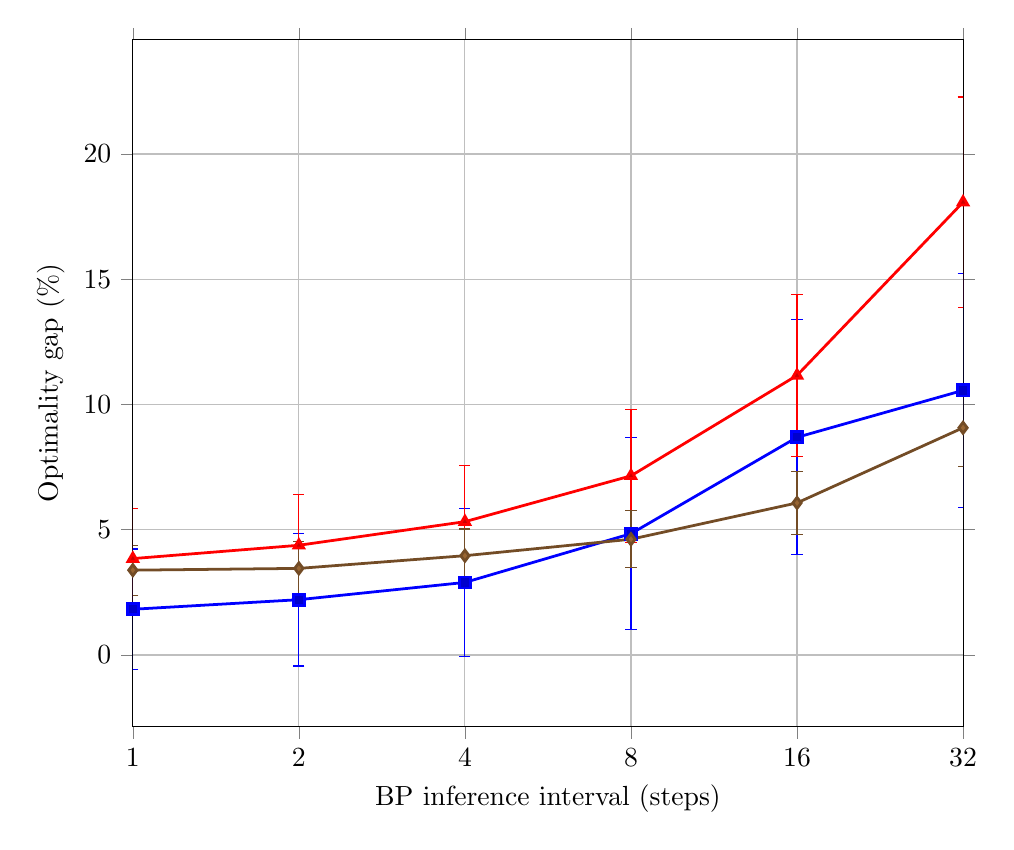
\begin{tikzpicture}
\begin{axis}[
  width=\linewidth, height=0.85\linewidth,
  xmode=log, log basis x={2},
  xmin=1, xmax=32,
  xtick={1,2,4,8,16,32},
  xticklabels={1,2,4,8,16,32},
  xlabel={BP inference interval (steps)},
  ylabel={Optimality gap (\%)},
  ymajorgrids, grid=both,
  tick align=outside,
  legend to name=sharedlegend,   % <-- share legend
  legend columns=2
]
  % MIS(n=100) (gap)
  \addplot+[
    mark=square*,
    line width=1pt,
    error bars/.cd, y dir=both, y explicit
  ] coordinates {
    (1, 1.824) +- (0, 2.405)
    (2, 2.207) +- (0, 2.646)
    (4, 2.896) +- (0, 2.957)
    (8, 4.842) +- (0, 3.830)
    (16, 8.688) +- (0, 4.694)
    (32, 10.563) +- (0, 4.664)
  };
  \addlegendentry{MIS ($n=100$)}

  % MIS(n=[200;300]) (gap)
  \addplot+[
    mark=triangle*,
    line width=1pt,
    error bars/.cd, y dir=both, y explicit
  ] coordinates {
    (1, 3.847) +- (0, 1.988)
    (2, 4.379) +- (0, 2.038)
    (4, 5.321) +- (0, 2.244)
    (8, 7.151) +- (0, 2.651)
    (16, 11.160) +- (0, 3.238)
    (32, 18.074) +- (0, 4.200)
  };
  \addlegendentry{MIS ($n\sim [200,300]$)}

  % Dataset B (gap)
  \addplot+[
    mark=diamond*,
    line width=1pt,
    error bars/.cd, y dir=both, y explicit
  ] coordinates {
    (1, 3.385  ) +- (0, 0.995 )
    (2, 3.456  ) +- (0, 1.058 )
    (4, 3.963  ) +- (0, 1.064 )
    (8, 4.62   ) +- (0, 1.131 )
    (16, 6.07   ) +- (0, 1.248 )
    (32, 9.07) +- (0, 1.56)
  };
  \addlegendentry{MIS ($n\sim [700,800]$)}
\end{axis}
\end{tikzpicture}
%\caption{Optimality gap}
\end{subfigure}
\hfill
% --- Right: Runtime ---
\begin{subfigure}{0.48\linewidth}
\centering
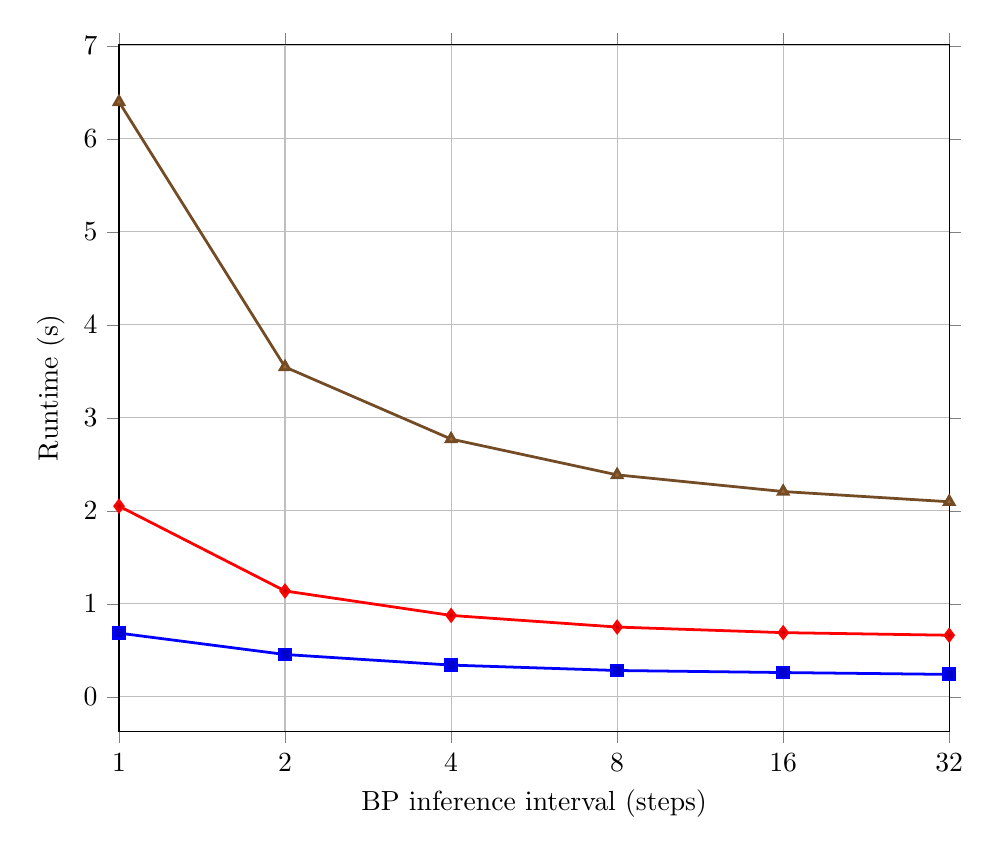
\begin{tikzpicture}
\begin{axis}[
  width=\linewidth, height=0.85\linewidth,
  xmode=log, log basis x={2},
  xmin=1, xmax=32,
  xtick={1,2,4,8,16,32},
  xticklabels={1,2,4,8,16,32},
  xlabel={BP inference interval (steps)},
  ylabel={Runtime (s)},
  ymajorgrids, grid=both,
  tick align=outside,
  %legend to name=sharedlegend,   % <-- same name
  legend columns=2
]
  % Dataset A (runtime)
  \addplot+[
    mark=square*,
    %dashed,
    line width=1pt
  ] coordinates {
    (1, 0.686) (2, 0.456) (4, 0.342)
    (8, 0.284) (16, 0.262) (32, 0.242)
  };
  %\addlegendentry{MIS ($n=100$)}

  % MIS (n=[200;300]) (runtime)
  \addplot+[
    mark=diamond*,
    %dashed,
    line width=1pt
  ] coordinates {
    (1, 2.051) (2, 1.139) (4, 0.876)
    (8, 0.751) (16, 0.691) (32, 0.663)
  };
  %\addlegendentry{MIS ($n\sim [200,300]$)}

  % MIS (n=[700;800]) (runtime)
  \addplot+[
    mark=triangle*,
    %dashed,
    line width=1pt
  ] coordinates {
    (1, 6.397) (2, 3.547) (4, 2.772)
    (8, 2.387) (16, 2.208) (32, 2.098)
  };
  %\addlegendentry{MIS ($n\sim [700,800]$)}
\end{axis}
\end{tikzpicture}
%\caption{Runtime}
\end{subfigure}

% --- Print shared legend once (after both axes are built)
\vspace{0.4em}
\pgfplotslegendfromname{sharedlegend}

\caption{Effect of BP inference frequency on (left) optimality gap and (right) runtime, with one shared legend. These values were obtained for the canonical probability model, the values of $\EPARAM$ were not learned.}
\label{fig:bp_gap_runtime_split}
\end{figure}


\begin{figure}[H]
\centering
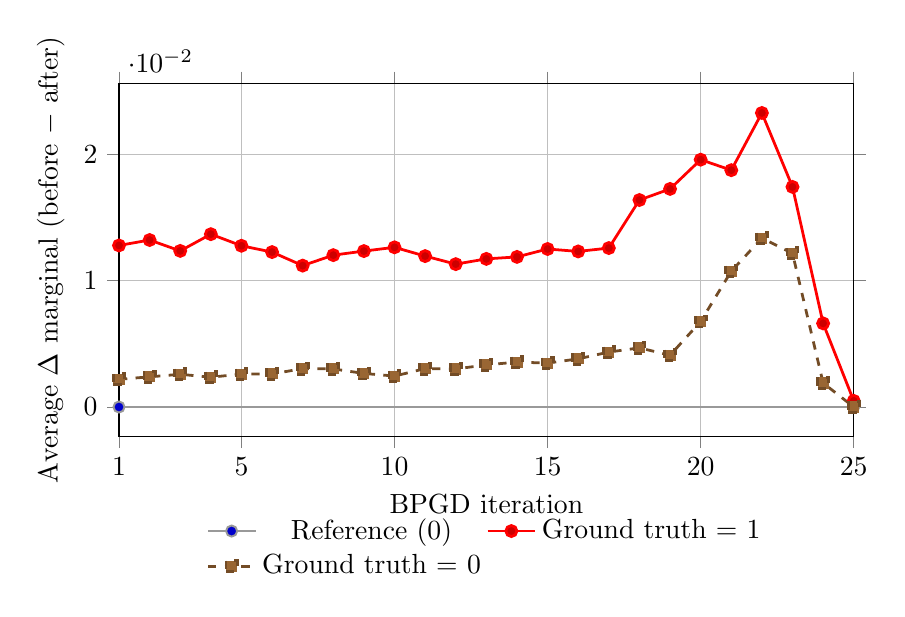
\begin{tikzpicture}
\begin{axis}[
  width=0.9\linewidth, height=0.5\linewidth,
  xlabel={BPGD iteration},
  ylabel={Average $\Delta$ marginal (before $-$ after)},
  xmin=1, xmax=25,
  xtick={1,5,10,15,20,25},
  ymajorgrids, grid=both,
  tick align=outside,
  legend columns=2,
  legend style={at={(0.5,-0.2)},anchor=north,draw=none,fill=none},
  % Uncomment next two lines if you prefer "improvement-positive" for GT=1:
  % yticklabel style={/pgf/number format/fixed},
  % y label style={align=center},
]
  % Zero reference
  \addplot+[smooth, domain=1:25, samples=2, line width=0.7pt, color=black!40] {0};
  \addlegendentry{Reference (0)}

  % === GT = 1 curve (your first vector) ===
  \addplot+[
    mark=*,
    line width=1pt,
  ] coordinates {
    (1, 0.01277997) (2, 0.01321043) (3, 0.01234875) (4, 0.01367217) (5, 0.01275521)
    (6, 0.01225579) (7, 0.01118489) (8, 0.01201370) (9, 0.01233569) (10, 0.01263245)
    (11, 0.01193830) (12, 0.01130253) (13, 0.01171802) (14, 0.01187442) (15, 0.01250025)
    (16, 0.01230669) (17, 0.01257457) (18, 0.01637567) (19, 0.01725165) (20, 0.01956591)
    (21, 0.01873445) (22, 0.02326167) (23, 0.01741204) (24, 0.00661565) (25, 0.00048573)
  };
  \addlegendentry{Ground truth = 1}

  % === GT = 0 curve (your second vector) ===
  \addplot+[
    mark=square*,
    dashed,
    line width=1pt,
  ] coordinates {
    (1, 0.00219178) (2, 0.00238550) (3, 0.00258879) (4, 0.00235593) (5, 0.00260759)
    (6, 0.00261363) (7, 0.00303784) (8, 0.00301133) (9, 0.00265429) (10, 0.00244694)
    (11, 0.00303629) (12, 0.00300891) (13, 0.00333170) (14, 0.00355504) (15, 0.00347144)
    (16, 0.00380908) (17, 0.00434687) (18, 0.00467745) (19, 0.00409546) (20, 0.00676624)
    (21, 0.01074063) (22, 0.01335998) (23, 0.01215781) (24, 0.00189862) (25, 0.00000000)
  };
  \addlegendentry{Ground truth = 0}
\end{axis}
\end{tikzpicture}
\caption{Average per-step change in marginals when clamping evidence during BPGD.
Positive values mean the marginal decreased after the update (since $\Delta=\text{before}-\text{after}$).
Curves are averaged over the test set.}
\label{fig:bpgd_delta_marginals}
\end{figure}


\subsection{Failure Modes: Feasible–Infeasible Overlap in Predicted Log-Potentials}
Figure~\ref{fig:violin-comparison} shows the predicted log-potentials $\hat{\theta}(x_F)$
for factor assignments, grouped by their feasibility.
Feasible assignments form a compact, high-scoring distribution
(centered closer to $0$), whereas most infeasible assignments are pushed to large negative values,
indicating low model probability.
However, we also observe a distinct island of \emph{infeasible} assignments with relatively high
log-probabilities that overlap the feasible region.
This suggests either that (i) the model has not fully captured the structural constraints
that separate these violating cases, or (ii) these assignments are genuinely hard—being
highly similar to feasible ones under the current featureization/parameterization.
Consequently, while the overall separation is encouraging, further refinement of the
model or features (e.g., stronger constraint-aware potentials, additional penalties,
or targeted negatives) may be required to reduce this overlap.

\begin{figure}[htbp]
    \centering
    \begin{subfigure}[b]{0.32\textwidth}
        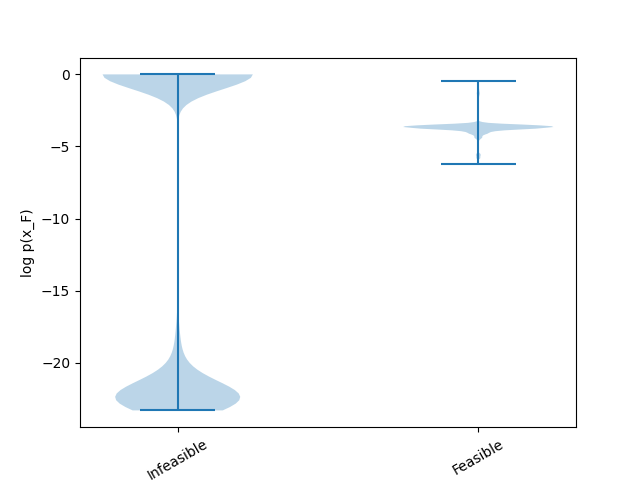
\includegraphics[width=\textwidth]{resources/img/violin_theta_factor/scp_n50_m50_k5.csv.png}
        \caption{$SCP\,(n=50, m=50, k=5)$}
        \label{fig:violin_scp_n50_m50_k5}
    \end{subfigure}
    \hfill
    \begin{subfigure}[b]{0.32\textwidth}
        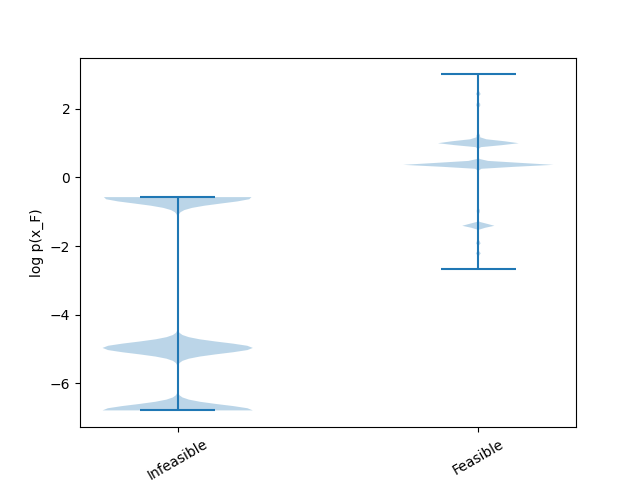
\includegraphics[width=\textwidth]{resources/img/violin_theta_factor/mis_n100_p0.15.csv.png}
        \caption{$MIS\,(n=100, p=0.15)$}
        \label{fig:violin_mis_n100_p0.15}
    \end{subfigure}
    \hfill
    \begin{subfigure}[b]{0.32\textwidth}
        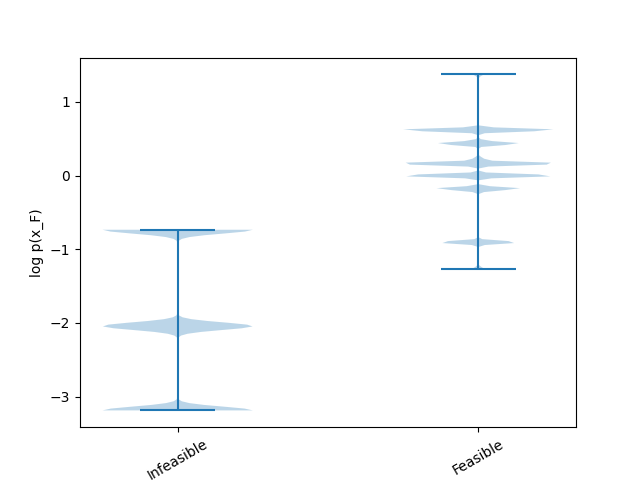
\includegraphics[width=\textwidth]{resources/img/violin_theta_factor/mis_n200:300_p0.15_maxdeg15.csv.png}
        \caption{$MIS\,(n\sim [200,300], p=0.15)$}
        \label{fig:violin_mis_n200:300_p0.15}
    \end{subfigure}
    \caption{Distributions of log-potentials $\EPARAMF(\XFACT)$ predicted by the GNN$+$LBP model and grouped by the feasibility of factor assignments. Overall, feasible assignments receive higher log-probabilities (near $0$) while infeasible ones are mostly suppressed (large negative values). Notably, an island of infeasible assignments attains unexpectedly high scores, overlapping the feasible region—indicating either remaining model misspecification or strong similarity between those infeasible assignments and feasible ones.}
    \label{fig:violin-comparison}
\end{figure}

\todo[inline]{add same violin plots for GNN+NMF models}



\subsection{Discussion}

Across MIS and SCP benchmarks, the main takeaway is clear: replacing factorized logits with an explicitly structured, differentiable MRF and decoding with BP-Guided Decimation (BPGD) systematically improves solution quality over a strong GNN-only baseline, at a modest but controllable runtime cost.

\paragraph{Solution quality.}
On SCP ($n{=}50,m{=}50,k{=}5$), our learned LBP$+$GD reduces the mean optimality gap from $10.92\%$ (GNN) to $1.54\%$ (Table~\ref{tab:lbp_nmf_bpgd_test_gap_results}), confirming that modeling dependencies among sets/items is particularly beneficial for covering constraints. The trend holds on MIS: for $n{=}100$ (ER graphs with $p{=}0.15$), LBP cuts the GNN gap from $14.55\%$ to $8.85\%$, and LBP$+$GD brings it further down to $6.92\%$; for larger MIS graphs ($n{\sim}[200,300]$) the improvement is even more pronounced, dropping from $22.85\%$ (GNN) to $4.71\%$ with LBP$+$GD. These gains are obtained despite fixing the number of BP iterations and using simple four-layer encoders, highlighting that the bulk of the advantage comes from enforcing local consistency through the factor graph.

\paragraph{Runtime–quality trade-off.}
The structured decoders are costlier than a pure greedy pass, but remain inexpensive in absolute terms on the sizes we target. On SCP ($50{\times}50$), moving from GNN ($0.06$s) to LBP$+$GD ($0.404$s) yields an order-of-magnitude reduction in gap for only a few extra tenths of a second (Table~\ref{tab:lbp_nmf_bpgd_test_time_results}). On MIS, LBP$+$GD roughly doubles to triples the runtime compared to GNN (e.g., $0.38$s $\rightarrow$ $0.85$s at $n{=}100$, and $0.98$s $\rightarrow$ $2.08$s at $n{\sim}\mathcal{U}[200,300]$), but delivers large gap reductions. Our frequency-ablation (Fig.~\ref{fig:bp_gap_runtime_split}) shows that running BP every $4$–$8$ decimation steps preserves most of the quality gains while shaving $30\%$–$50\%$ of decoding time, offering a practical knob for deployment under time budgets.

\paragraph{Effect of evidence and guidance.}
BPGD’s advantage over one-shot greedy decoding stems from the ability to clamp partial assignments and re-propagate their impact through constraints. Fig.~\ref{fig:bpgd_delta_marginals} quantifies this: the average change in marginals is small early on (when evidence is weak) and grows later, when conflicts and coverage become decisive. This adaptivity specifically mitigates tie-breaking failures of score-guided greedy methods in mutually exclusive neighborhoods (MIS) and in overlapping, high-coverage sets (SCP).

\paragraph{Comparison to “train-less” canonical MRFs.}
Using hand-crafted canonical parameters (zero for feasible configurations, $-\infty$ for infeasible) with BPGD provides a strong unsupervised baseline (Table~\ref{tab:canonical_mrf_gap_results}). On SCP, our learned LBP$+$GD ($1.54\%$) clearly surpasses canonical LBP$+$GD ($4.03\%$), indicating that parameter learning captures instance-specific structure beyond feasibility. On MIS, the canonical LBP$+$GD is competitive or better at the current capacity/feature budget (e.g., $1.82\%$ vs.\ $6.92\%$ at $n{=}100$, $3.85\%$ vs.\ $4.71\%$ at $n{\sim}\mathcal{U}[200,300]$), suggesting that (i) MIS with pairwise factors already benefits greatly from feasibility propagation, and (ii) our learned parameterization still has headroom—richer embeddings, better calibration of pairwise potentials, or curriculum schedules for BP could close this gap. Importantly, both learned and canonical NMF variants underperform LBP, which aligns with our analysis of mean-field’s inability to reflect degree/overlap effects under homogeneous canonical parameters.

\paragraph{Scalability and limits.}
Even with loopy graphs and fixed iteration budgets, LBP remains stable in practice and scales gracefully in our regime. Absolute solve times stay within seconds on a single GPU and grow smoothly with $n$ (Tables~\ref{tab:lbp_nmf_bpgd_test_time_results},~\ref{tab:canonical_mrf_gap_results}). The main limitations we observe are (i) sensitivity to the number of BP iterations and damping, and (ii) the expressivity/size trade-off of the exponential-family parameterization with over-complete statistics (which grows with factor size). These constraints motivated our focus on MIS and SCP, where factor arity is controlled; generalizing to problems with large or learned higher-order factors will require either structured parameter tying or low-rank/sparse parameterizations.

\section{Conclusion}
It is important to emphasize that the present study was designed primarily to highlight the improvements brought by structured inference (BP) compared to factorized logit predictions. To make this comparison clear and tractable, we deliberately focused on problem families (MIS and SCP) whose natural formulations yield factor graphs with small arity. In this setting, the canonical over-complete parametrization is still feasible to implement, and thus we can study the effect of inference in a controlled environment. Future contributions will move beyond this “idealized” parametrization to problems involving larger factors, where the exponential growth of sufficient statistics makes canonical representations impractical. This shift will require approximate parameterizations, structured factor tying, or low-rank formulations, and will allow us to test the generality of MRF-augmented predictors in more realistic combinatorial optimization tasks.

\paragraph{Take-home messages.}
(i) Structured, differentiable inference (LBP) coupled with BPGD reliably improves over factorized GNN predictors on both packing and covering problems; (ii) the extra cost is small and can be tuned via the BP-frequency knob; (iii) canonical “train-less” MRFs form a strong baseline on MIS, but learning clearly helps on SCP and should help more broadly as parameterizations and features are enriched; and (iv) naïve mean-field is ill-suited here, whereas LBP effectively communicates exclusivity/coverage through the graph. Overall, the results validate MRF-augmented learning as a practical path to higher-quality, feasible solutions in CO, and motivate future work on (a) stronger parameter heads (e.g., degree-aware or message-calibrated potentials), (b) adaptive inference schedules (entropy/variance-triggered updates), and (c) scalable approximations for higher-order factors.



